\documentclass[tufte-handout]{standalone}
\usepackage{mathpazo} % Sets Palatino as the main font
\usepackage{tikz}
\usetikzlibrary{3d, angles, quotes, calc, backgrounds}
\usetikzlibrary{decorations.markings,shapes.geometric, arrows, positioning}

% my colors
\definecolor{darkslategray}{rgb}{0.18, 0.31, 0.31}
\definecolor{myorange}{rgb}{0.89804, 0.55686, 0.19608}

\tikzstyle{root} = [ellipse, rounded corners, minimum width=2cm, minimum height=1.5cm,text centered, draw=black!90, thick, fill=darkslategray, text=white]
\tikzstyle{first} = [rectangle, rounded corners, minimum width=3cm, minimum height=1cm, text centered, fill=darkslategray!20, draw=darkslategray!80!black, font=\bfseries\itshape]
\tikzstyle{second} = [rectangle, rounded corners, minimum width=3cm, minimum height=1cm, text centered, fill=myorange!20, draw=myorange!80!black, font=\bfseries]
\tikzstyle{third} = [rectangle, rounded corners, minimum width=1.5cm, minimum height=1cm, text centered, fill=myorange!5, draw=myorange!80!black, font=\itshape]
\tikzstyle{arrow} = [thick,->,>=stealth]
\tikzstyle{line} = [thick,-,>=stealth]

\begin{document}

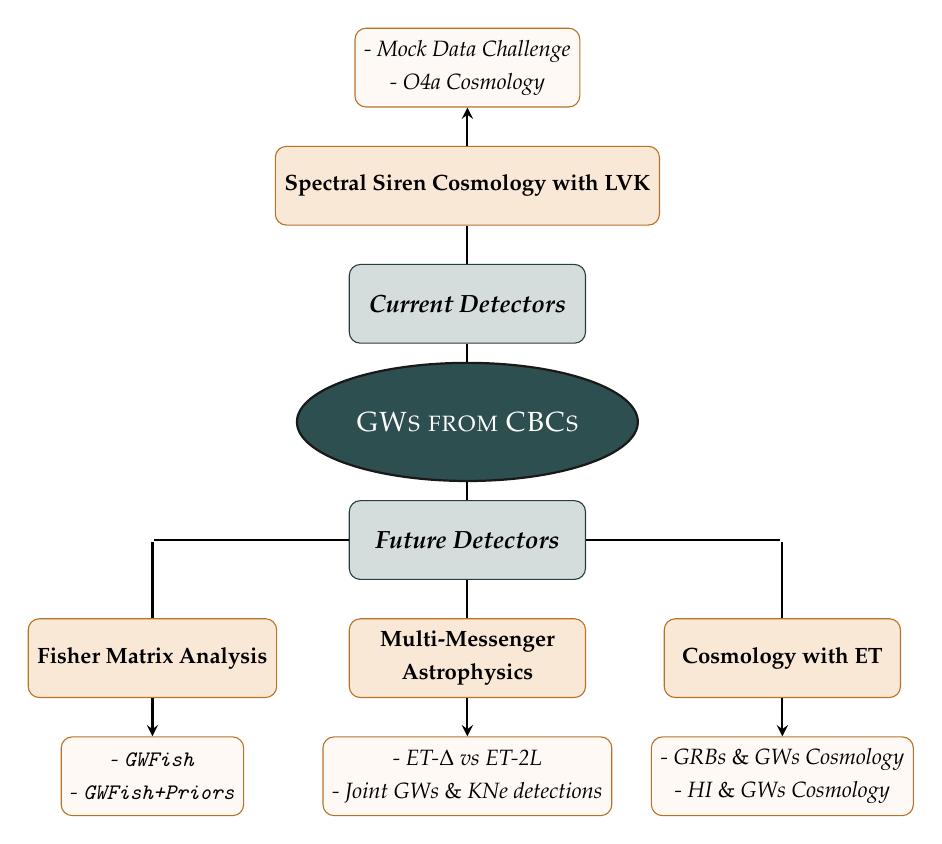
\begin{tikzpicture}[node distance=1.5cm, every node/.style={fill=white}, align=center]

% Main script
\node (main) [root] {{\textsc{GWs from CBCs}}};

\node (currentDet) [first,above of=main] {\small{Current Detectors}};
\node (futureDet) [first,below of=main] {\small{Future Detectors}};

\node (spectral) [second, above of=currentDet] {\footnotesize{Spectral Siren Cosmology with LVK}};
\node (spectralWorks) [third, above of=spectral] {\footnotesize{- Mock Data Challenge}\\\footnotesize{- O4a Cosmology}};

\node (data) [second, left of=futureDet, yshift=-1.5cm, xshift=-2.5cm] {\footnotesize{Fisher Matrix Analysis}};
\node (dataWorks) [third, below of=data] {\footnotesize{- \texttt{GWFish}}\\\footnotesize{- \texttt{GWFish+Priors}}};

\node (mm) [second, below of=futureDet] {\footnotesize{Multi-Messenger}\\\footnotesize{Astrophysics}};
\node (mmWorks) [third, below of=mm] {\footnotesize{- ET-$\Delta$ vs ET-2L}\\\footnotesize{- Joint GWs $\&$ KNe detections}};

\node (cosmo) [second, right of=futureDet, yshift=-1.5cm, xshift=2.5cm] {\footnotesize{Cosmology with ET}};
\node (cosmoWorks) [third, below of=cosmo] {\footnotesize{- GRBs $\&$ GWs Cosmology}\\\footnotesize{- HI $\&$ GWs Cosmology}};

\draw[line] (main)  -- (currentDet);
\draw[line] (main)  -- (futureDet);



%\draw[line] (currentDet) -- node[above of=currentDet, yshift=-1.5cm, execute at begin node = \setlength{\baselineskip}{0.2em}] {\scriptsize{\textit{Chapter 2}}} (spectral);
\draw[line] (currentDet) -- (spectral);
\draw[arrow] (spectral)  -- (spectralWorks);

\node (anchor1) [inner sep=0pt, left of=futureDet, xshift=-2.5cm]{};
\node (anchor2) [inner sep=0pt, right of=futureDet, xshift=2.5cm]{};

\draw[line] (futureDet) -- (anchor1);
\draw[line] (futureDet) -- (anchor2);

\draw[line] (anchor1) -- (data);
\draw[line] (futureDet) -- (mm);
\draw[line] (anchor2) -- (cosmo);

\draw[arrow] (data) -- (dataWorks);
\draw[arrow] (mm) -- (mmWorks);
\draw[arrow] (cosmo) -- (cosmoWorks);


\end{tikzpicture}

\end{document}
